In current academic documents figures and tables are key sources of information, i.e. taking a look at a table in a paper can quickly summarize the work that has been done.
However, these are not currently used in academic search engines.
To better answer any kind of question the use of figure and tables is encouraged.

When there is a focus on scientific papers, it has been shown that \textbf{captions} are the key elements to indentify figures and tables.
The difference between body text and captions has been proven to relatively easy to detect \cite{pdffigures2}.
The search is done by looking for keywords that are likely to start a caption.
Afterwards false positives are removed by applying a filter to them.
This filter is focused on a particular format convention.
This process of these filters is repeated until no false positives remain.

The second step is to classify every part of the paper as a certain region: caption, body text, graphical element or figure text.
Caption regions are made from the captions and the following lines of text (if there are any).
\href{https://poppler.freedesktop.org/}{Poppler's algorithm} is used to define body text or figure text.
Additional heuristics are applied for improved accuracy. 
To find the graphical elements, the pdf is directly parsed. 
Internally PDF's make use of various ``operators'' that draw elements on the page. 
The algorithm uses the bounding boxes defined by the operators that the PDF would use to draw.
The boxes can be merged if required to form the complete graphical region.
An example of this can be seen in Figure \ref{fig:pdffigure}.

\begin{figure}
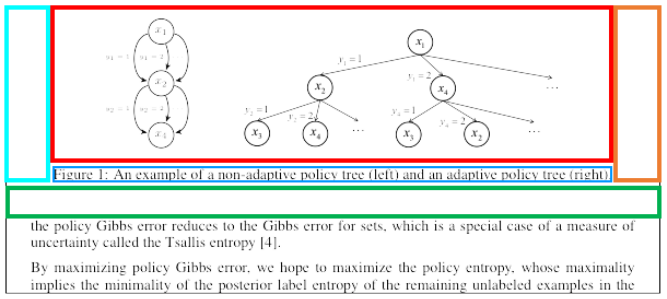
\includegraphics[width=0.48\textwidth]{pdffigures}
\caption{An example of seperation into regions}\label{fig:pdffigure}
\end{figure}


To assign captions/titles to figures or tables clustering is utilized. 
These clusters would be pruned and additional rules for increased performance.
Questions that would match up with elements in a caption can now be linked to a corresponding image which might contain useful information to answer the question.

